\documentclass[tikz]{standalone}

\colorlet{FilledSurface}{blue!20}
\colorlet{FilledSurfaceGroupOne}{blue!20}
\colorlet{FilledSurfaceGroupTwo}{red!20}
\colorlet{FilledSurfaceGroupThree}{green!20}
\colorlet{FilledSurfaceGroupFour}{magenta!20}
\colorlet{FormulaBackground}{green!10}
\colorlet{FormulaFrame}{green}


\usetikzlibrary{calc}
\usepackage{tikz-dimline}

\begin{document}
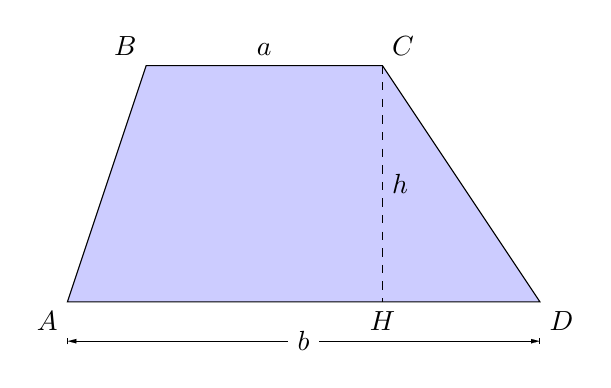
\begin{tikzpicture}

\coordinate (A) at (0, 0);
\coordinate (B) at (1, 3);
\coordinate (C) at (4, 3);
\coordinate (D) at (6, 0);
\draw[fill=FilledSurfaceGroupOne]
    (A) node[below left]{$A$}
    -- (B) node[above left]{$B$}
    -- node [above]{$a$} (C) node[above right]{$C$}
    -- (D) node[below right]{$D$}
    -- cycle;

\coordinate (H) at ($(A)!(C)!(D)$);
\node [below] at (H) {$H$};
\draw[dashed](C) -- (H) node [midway, right] {$h$};

\dimline[extension start length=0, extension end length=0]
        {($(A)!.5cm!-90:(D)$)}
        {($(D)!.5cm!90:(A)$)}
        {$b$};

\end{tikzpicture}
\end{document}

